\documentclass[10pt,showpacs,preprintnumbers,amsmath,amssymb,nofootinbib,aps,prl,twocolumn,groupedaddress,superscriptaddress,showkeys]{revtex4-1}
\usepackage{graphicx}
\usepackage{dcolumn}
\usepackage{bm}
\usepackage[colorlinks=true,urlcolor=blue,citecolor=blue]{hyperref}
\usepackage{color}
\usepackage{listings}
\usepackage{subfig}
\usepackage{float}
\usepackage{tikz} % Send help 
\usepackage{physics}


\lstset{ %
  basicstyle=\footnotesize,        % the size of the fonts that are used for the code
  breakatwhitespace=false,         % sets if automatic breaks should only happen at whitespace
  breaklines=true,                 % sets automatic line breaking
  captionpos=t,                    % sets the caption-position to bottom
  deletekeywords={...},            % if you want to delete keywords from the given language
  escapeinside={\%*}{*)},          % if you want to add LaTeX within your code
  extendedchars=true,              % lets you use non-ASCII characters; for 8-bits encodings only, does not work with UTF-8
  frame=single,                    % adds a frame around the code
  keepspaces=true,                 % keeps spaces in text, useful for keeping indentation of code (possibly needs columns=flexible)
 % language=Python,                 % the language of the code
  morekeywords={*,...},           % if you want to add more keywords to the set
  numbers=left,                    % where to put the line-numbers; possible values are (none, left, right)
  numbersep=5pt,                   % how far the line-numbers are from the code
  showspaces=false,                % show spaces everywhere adding particular underscores; it overrides 'showstringspaces'
  showstringspaces=false,          % underline spaces within strings only
  showtabs=false,                  % show tabs within strings adding particular underscores
  stepnumber=1,                    % the step between two line-numbers. If it's 1, each line will be numbered
  tabsize=2,                       % sets default tabsize to 2 spaces
}

\newcommand{\lexp}{\ket{\downarrow}}
\begin{document}
\title{FYS3150 Computational Physics - Project 4}
\author{Nicholas Karlsen}


\begin{abstract}
  Using the Metropolis algorithm to study a system of coupled paramagnets, the Ising model. Derived exact solutions of expectation values for a 2 by 2 lattice and found the algorithm to make accurate predictions to the third decimal in $10^6$ Monte Carlo cycles. Further, looked at a 20 by 20 lattice and found a link between the equilibration time and the temperature of the system. Lastly, tried to observe the phase transition, and replicate the result produced by \textcite{PhysRev.65.117}, observed the expected behavior qualitatively, but failed to extract numbers.
\end{abstract}

\maketitle


\section{Introduction}

In this report, we will look at the Ising model, a model describing locally coupled paramagnets and how this model can be studied numerically using the Metropolis Monte Carlo algorithm, which in short emulates the time-development of the system using statistics and random numbers. 

The model has analytic solutions for a 2-Dimensional lattice, which will be used as a way of testing the code. These analytic predictions include expectation values for the $2\times2$ lattice, as well as the critical temperature, when the system undergoes a phase transition which in the thermodynamic limit where $L\rightarrow \infty$ was first derived analytically by \textcite{PhysRev.65.117}

The programs accompanying this report were written in python, and can be found on my github \url{https://github.com/nicholaskarlsen/FYS3150/tree/master/Project_4}.

\section{Theory, Algorithms and Methods}
  \subsection{The Ising Model}
    The Ising model aims to model a lattice of magnetic dipoles, and can be thought of as an extension to the ideal paramagnet, by looking at the local interaction between directly neighboring spins (See fig. \ref{fig:spinsites}), such that the energy of the system is instead proportional to the sum of the interactions of all coupled spins, which gives a more accurate description of the system compared to the simple case of an ideal paramagnet and makes predictions of phase transitions for dimensions greater than one.

    The lattice energy in a system described by the Ising model with no external fields is given by Eqn.~\ref{eqn:ising_energy}, where $s_i \in \{-1, 1\}$ and $J$ is a coupling constant, within which is contained type of the coupling. For this project we will look at $J=1$, which corresponds to a ferromagnetic coupling.

    \begin{equation}
      E = -J\sum_{<kl>} s_ks_l
      \label{eqn:ising_energy}
    \end{equation}
    In this sum, the notation $<kl>$ means that we take the sum over each coupling $s_k s_l$.
    Consider again Fig.\ref{eqn:ising_energy}. The contribution, $\epsilon_i$, to the total energy due the interactions at spin-site $i$ is the sum of its interactions, $\epsilon_i = s_i(s_\uparrow + s_\downarrow + s_\leftarrow + s_\rightarrow)$ where the arrows denote the spin-site directly neighboring site $i$ in the direction of the arrow. Now wish to compute the energy contribution due to the interactions at the spin-site left of site $i$. In this case, the interaction between it, and spin-site $i$ has already been computed, and must not be counted again.

    \begin{figure}[H]
      \centering
      \begin{tikzpicture}
        [%%%%%%%%%%%%%%%%%%%%%%%%%%%%%%
        dot/.style={circle,draw=black, fill,inner sep=1pt},
        ]%%%%%%%%%%%%%%%%%%%%%%%%%%%%%% 
        \foreach \x in {-1,...,3}{
          \foreach \y in {-1,...,3}{
            % Draw 3x3 dot lattice
            \node[dot] at (\x,\y){};
            \node[dot] at (\x,\y){};
          }
        }
        \draw[thick, dashed] (1 + .1 , 1) -- (1 + 0.9, 1);
        \draw[thick, dashed] (1 - .1 , 1) -- (1 - 0.9, 1);
        \draw[thick, dashed] (1, 1 + .1) -- (1, 1 + 0.9);
        \draw[thick, dashed] (1, 1 - .1) -- (1, 1 - 0.9);
        % Text 
        \draw (1+.25, 1+.2) node{$s_{i}$};
      \end{tikzpicture}
      \caption{Section of a 2D lattice, where each spin-site is represented by a dot. In the Ising model, spin-site $i$ will only interact with its directly neighboring spin-sites, indicated by dotted lines in this diagram\label{fig:spinsites}}
    \end{figure}

    Further, in this project the lattice will be treated as pseudo-continuous where any spin-sites located at an edge, will also interact with the spin-site on the opposing edge, illustrated in Fig.~\ref{fig:ising_periodic bounds}, which strictly speaking constitutes having periodic boundary conditions. If instead we had fixed boundary conditions, there would simply be no such across-lattice interactions, and spin-sites located at the edges would then only interact with 3 other spin-sites (2 in the case of corner sites) in the 2D case.
      \begin{figure}[H]
      \centering
      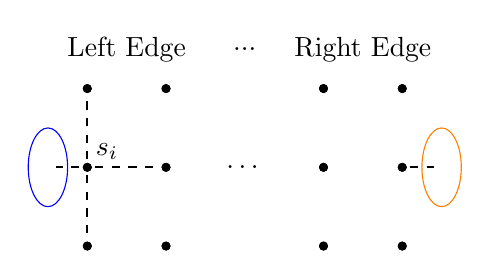
\begin{tikzpicture}
        [%%%%%%%%%%%%%%%%%%%%%%%%%%%%%%
        dot/.style={circle,draw=black, fill,inner sep=1pt},
        ]%%%%%%%%%%%%%%%%%%%%%%%%%%%%%% 
        \foreach \x in {2,...,1}{
          \foreach \y in {-1,...,1}{
            % Draw 3x3 dot lattice
            % LEFT LATTICE
            \node[dot] at (-\x,\y){};
            \node[dot] at (-\x,\y){};
            % RIGHT LATTICE
            \node[dot] at (\x,\y){};
            \node[dot] at (\x,\y){};
          }  
        }    
        % Lines
        \draw[thick, dashed] (-2, 0 + .1) -- (-2, 1 - .1);
        \draw[thick, dashed] (-2, 0 - .1) -- (-2, -1 + .1 );
        \draw[thick, dashed] (-2 + .1, 0) -- (-1 - .1, 0);

        \draw[color=blue] (-2.5,0) ellipse (0.25cm and .5cm);
        % Portal lines
        \draw[thick, dashed] (-2 - .1, 0) -- (-2.5 + .1, 0);
        \draw[thick, dashed] (2 + .1, 0) -- (2.5 - .1, 0);
        \draw[color=orange] (2.5,0) ellipse (0.25cm and .5cm);
        % Text
        \draw (0, 0) node{$\dots$};
        \draw (-1.5, 1.5) node{Left Edge};
        \draw (1.5, 1.5) node{Right Edge};
        \draw (0, 1.5) node{...};
        \draw (-2+.25, 0+.2) node{$s_{i}$};
      \end{tikzpicture}
      \caption{Spin-site $i$, located at the left edge of the lattice interacting with its direct neighbors, as well as the spin site on the opposite edge of the lattice
      \label{fig:ising_periodic bounds}}
    \end{figure}

    Much simpler, the net magnetization, $\mathcal M$, of the system is taken as the sum over all spins
    \begin{equation*}
      \mathcal M = \sum_i s_i
    \end{equation*}
    Howver, the magnetization, is quite unstable and will frequently oscillate about $0$ in the region of temperatures which will be studied, as seen in Fig.~\ref{fig:net_magnetization}, a select result from one of the simulations to be discussed later. As such, we will instead look at the absolute value of the net magnetization, as it will provide more stable results that are easier to interpret.
    \begin{figure}[H]
      \centering
      \includegraphics[width=8cm]{figs/ex_e_M.pdf}
      \caption{\label{fig:net_magnetization}Net magnetization as a function of temperature, simulated with $2\cdot10^6$ Monte Carlo cycles}
    \end{figure}


    \subsubsection{Boltzmann Statistics}
      From this model we can derive many thermodynamic quantities by the use of Boltzmann statistics, where we have the probability of the system being in some specific state at temperature\footnote{Contained within $\beta$ in this notation}
      \begin{equation}
        \mathcal P(E_s) = \frac{1}{Z} e^{-\beta E_s}
      \end{equation}
      With $\beta \equiv \frac{1}{k_B T}$, the thermodynamic beta and $Z$, the partition function, acting as a normalization factor given by

      \begin{equation}
        Z = \sum_s e^{-\beta E_s}
        \label{eqn:partition function}
      \end{equation}
      From this, the expectation value of some quantity $X$, with micro-states $X_s$ can be computed by

      \begin{equation}
        \left<X\right> = \sum_s X_s \mathcal P(E_s) = \frac{1}{Z} \sum_s X_s e^{-\beta E_s} 
        \label{eqn:expecval}
      \end{equation}
      Using this, we can compute the specific heat capacity, $C_V$ by computing the expectation values of $E, E^2$ \cite{statmek_lecnotes}, related by the following expression

      \begin{equation}
        C_V = \frac{\left<E^2\right> - \left<E\right>^2}{k_B T^2}
        \label{eqn:speciffic heat}
      \end{equation}
      Where $\left<X^2\right> - \left<X\right>^2$ is recognized as the variance of a set of randomly distributed quantities, $\sigma_X^2$.

      In a similar fashion, the magnetic susceptibility\footnote{Using the absolute magnetization to compute $\chi$, in line with the problem text for 4e}, $\chi$, is calculated from $\sigma_{\mathcal |M|} ^2$ \cite{statmek_lecnotes}

      \begin{equation}
        \chi = \frac{\sigma^2_\mathcal{|M|}}{k_B T}
        \label{eqn:suceptibility}
      \end{equation}

      For more details on the Ising model, or Boltzmann statistics refer to \textcite[Ch~6, 8.2]{schroeder}, \textcite{statmek_lecnotes}, or similar texts on the topic.

  \subsubsection{Analytic solution of 2x2 Lattice}
    Consider now a $2\times2$ lattice, each with spin $\pm 1$.
    The energy of the system for a particular micro-state is given by Eqn.~\ref{eqn:ising_energy}, so for a $2\times2$ lattice we have

    \begin{equation}
      E = -J\sum_{<kl>}s_{kl} = -J\qty( 2s_1s_2 + 2s_1s_3 + 2s_2s_4 + 2s_3s_4)
    \end{equation}
    The multiplicity, that is number of possible combinations of micro-states for a system consisting of 4 spins is $2^4=16$.

     \begin{figure}[H]
      \centering
      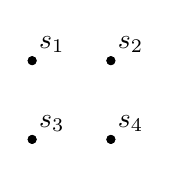
\begin{tikzpicture}
        [%%%%%%%%%%%%%%%%%%%%%%%%%%%%%%
        dot/.style={circle,draw=black, fill,inner sep=1pt},
        ]%%%%%%%%%%%%%%%%%%%%%%%%%%%%%% 
        \foreach \x in {0,...,1}{
          \foreach \y in {0,...,1}{
            % Draw 3x3 dot lattice
            \node[dot] at (\x,\y){};
            \node[dot] at (\x,\y){};
          }
        }
        \draw (0+.25, 1+.2) node{$s_{1}$};
        \draw (1+.25, 1+.2) node{$s_{2}$};
        \draw (0+.25, 0+.2) node{$s_{3}$};
        \draw (1+.25, 0+.2) node{$s_{4}$};

      \end{tikzpicture}
      \caption{A $2\times2$ lattice of spin-sites}
    \end{figure}

    If we first consider the micro-state in which all the spins are in parallel, we get energy $E=-8J$. Thus, this particular macro-state is at least 2-fold degenerate\footnote{Two micro-states corresponds to the same observable macro-state.}.
    The different micro-states and their degeneracies are summed up in table \ref{tab:2x2energies} from \textcite{statmek_lecnotes}

    \begin{table}[H]
      \centering
      \caption{\label{tab:2x2energies} Possible configurations of 2x2 lattice}
      \begin{tabular}{llrr}
        No. spin up & Degeneracy & $E$ & $\mathcal M$ \\ \hline
        4 & 1 & -8J & 4 \\
        3 & 4 & 0 & 2 \\
        2 & 4 & 0 & 0 \\
        2 & 2 & 8J & 0 \\
        1 & 4 & 0 & -2 \\
        0 & 1 & -8J & -4 \\ \hline
      \end{tabular}
    \end{table}

    See that there are only 3 distinct energy macro-states, $E=-8J, 0, 8J$ corresponding to $2, 12$ and $2$ of the possible micro-states respectively.

    It is then easy to see from Eqn.~\ref{eqn:partition function} that the partition function for the system will take the following form
    \begin{equation}
      Z = 2e^{+8J\beta} + 2e^{-8J\beta} + 12 = 4\cosh(8J\beta) + 12
    \end{equation}

    From this, we derive analytic values for $\langle E \rangle, \langle |\mathcal M| \rangle , C_V$ and $\chi$. 

    First, compute the expectation value of the energy using an alternate, simpler expression from \textcite[Ch~6.2]{schroeder}

    \begin{equation}
      \langle E \rangle = -\frac{1}{Z}\pderivative{\beta}Z = -\frac{8J\sinh(8J\beta)}{\cosh(8J\beta) + 3}
    \end{equation}
    Similarly, the expectation value of $E^2$ is computed easily by another expression found in \textcite[Ch~6.2]{schroeder}
    \begin{equation}
      \langle E^2 \rangle = -\frac{1}{Z}\frac{\partial^2}{\partial\beta^2}Z = \frac{64J^2 \cosh(8J\beta)}{\cosh(8J\beta) + 3}
    \end{equation}
    From this, we can compute the variance of $E$
    \begin{align}
      \begin{split}
        \sigma_E^2 &= \langle E^2 \rangle - \langle E \rangle ^2 
      \end{split}
    \end{align}
    With which we can compute $C_V$ using Eqn.~\ref{eqn:speciffic heat}. Compute expectation values of $|\mathcal M|, |\mathcal M|^2$ using Eqn.~\ref{eqn:expecval} and Table~\ref{tab:2x2energies}

    \begin{align}
      \begin{split}
        \langle |\mathcal M | \rangle &= \frac{1}{Z} \sum_s |\mathcal M_s | e^{-\beta E_s} 
          \\
        &= \frac{8e^{8J\beta} + 16e^0}{Z} 
          \\
        &= \frac{2e^{8J\beta} + 4}{\cosh(8J\beta) + 3}
      \end{split}
    \end{align}

    \begin{align}
      \begin{split}
        \langle |\mathcal M |^2 \rangle &= \frac{1}{Z}\sum_s|\mathcal M_s|^2e^{-\beta E_s} 
          \\
        &= \frac{1}{Z}\qty(32e^{8J\beta} + 32e^{0}) 
          \\
        &= \frac{8e^{8J\beta} + 8}{\cosh(8J\beta) + 3}
      \end{split}
    \end{align}
    We can then compute the variance of the absolute net magnetization
    \begin{align}
      \begin{split}
        \sigma_{|\mathcal M|}^2 &= \langle |\mathcal M|^2\rangle - \langle |\mathcal M|\rangle^2
      \end{split}
    \end{align}
    Which can be used to compute the magnetic susceptibility using Eqn~\ref{eqn:suceptibility}.

    In table \ref{tab:2x2expec} we have the analytic results for the $2\times2$ lattice for $T=1$ in units where $J=1$, $k_B=1$.

    \begin{table}[H]
      \centering
      \caption{\label{tab:2x2expec} Analytic values for $T=1$}
      \begin{tabular}{r|r}
        $\langle E \rangle / L^2$ & -1.99598209\\
        $\langle |\mathcal M| \rangle / L^2$ & 0.9986607 \\
        $ C_v / L^2$ &  0.03208233 \\
        $\chi / L^2$ & 0.00401074 \\

      \end{tabular}
    \end{table}

    \subsubsection{Phase Transitions}
      As mentioned in the introduction, the 2-Dimensional Ising model was solved in the thermodynamic limit by \textcite{PhysRev.65.117}. Which predicts a phase-transition for a lattice of size $L\rightarrow \infty$ at curie temperature $T_C \approx 2.269$ in our dimensionless units \cite{project4}. 

      This temperature, is related to a finitely sized lattice by the following \cite{project4}
      \begin{equation}
        T_C(L) - T_C(L=\infty) = aL^{-1/\nu}
        \label{eqn:T_C(L) - T_C(L=infty)}
      \end{equation}
      Where $a$ is a constant of proportionality, and $\nu$ is a number related to the correlation length of the system \cite{project4}, which is set to $1$ for this project.

      A simple property that will change after the phase transition, that is when $T > T_C$, is that a ferromagnet will no longer exhibit spontaneous magnetization, As such, the magnetization will go to $0$ when $T\geq T_C$ when there is no external field present.

      For more, see \textcite{statmek_lecnotes}.


  \subsection{The Metropolis Algorithm}
    The metropolis algorithm is a type of Monte Carlo simulation, that is an algorithm where the system is sampled in a random way. The metropolis algorithm belongs to a family of Markov Chain Monte carol methods which simulate the time-evolution of stochastic systems.

    Specifically, for our system we pick $L^2$ spin-sites in the lattice for each Monte Carlo cycle, or sweep of the lattice.
    For each sample, we then perform the metropolis algorithm, which qualitatively evaluates the current state of the system, then evaluates the system if the spin of the current spin-site were to change. The likeliest state of the system is then chosen, and the energy and magnetization of the system is updated accordingly.

    Or more precisely

    \begin{enumerate}
      \item For each Monte Carlo cycle, sample $L^2$ random spin-sites.
      \item Compute the change in energy $\Delta$E due to flipping the spin
      \item If $\Delta E\leq 0$, set this as the new state of the system, and sample a new state.
      \item Else, If $\Delta E < 0$ compute $w = e^{-\beta\Delta E}$, If $w \geq r$, where $r$ is a random number in the interval $[0, 1)$, accept the flipped state, and sample a new one.
      \item If neither of the prior two statements are true, the system remains in its current state and a new sample is chosen.
    \end{enumerate}

    Afterwards, the expectation values are computed from the sums of all the states divided by the number of Monte Carlo cycles.

    Further, because computing $w$ is expensive, this algorithm is effectivized by pre-computing the possible energy changes of the system of which there are only 5, as shown in \textcite{statmek_lecnotes}.


  \begin{figure*}[h!p]
    \centering
    \subfloat[][]{
      \includegraphics[width=8cm]{figs/exc_E_1.pdf}
    }    
    \subfloat[][]{
      \includegraphics[width=8cm]{figs/exc_E_2.pdf}
    }
    \\
    \subfloat[][]{
      \includegraphics[width=8cm]{figs/exc_M_1.pdf}
    }    
    \subfloat[][]{
      \includegraphics[width=8cm]{figs/exc_M_2.pdf}
    }
    \\
    \subfloat[][]{
      \includegraphics[width=8cm]{figs/exc_count_1.pdf}
    }    
    \subfloat[][]{
      \includegraphics[width=8cm]{figs/exc_count_2.pdf}
    }
    \caption{\label{fig:20x20 expecvals} Expectation values computed for different numbers of Monte Carlo cycles for an ordered initial state of spin-ups and random initial state, different for each computed expectation value.}
  \end{figure*}
  \section{Results and Discussions}

  \subsection{Testing algorithm, L=2}

  In order to test the functionality, and consistency of the algorithm a $2\times2$ lattice with an initial state of all spin-ups was simulated 100 times each for a range of Monte Carlo cycles. The results for which are shown\footnote{Had some issues with figure placements, and no time to redo the report in something simpler to deal with than Revtex, so please excuse the poor placement of the larger figures.} in Fig.~\ref{fig:convergence 2x2}. If we disregard the results for $N=10$ Monte Carlo cycles, we see that the standard deviation of the output seems shrink in an approximately linear fashion with the logarithm of the number of Monte Carlo cycles. In particular, we see that for $10^6$ Monte Carlo cycles we have a standard deviation of $\sim10^{-4}$ meaning the algorithm outputs values consistent to the third decimal, and matches the theoretical result.

  \begin{figure}[H]
    \centering
    \subfloat[][]{
      \includegraphics[width=7cm]{figs/ex_d_histo_1.pdf}
    }

    \subfloat[][]{
      \includegraphics[width=7cm]{figs/ex_d_histo_2.pdf}
    }
    \caption{\label{fig:histo}Normalized histograms showing the relative no. occurrences of each energy in an equilibration time of $10^3$ Monte Carlo cycles for $T=\{1, 2.4\}$.}
  \end{figure}
  \subsection{Further investigations of the Ising model}

  Then, moving on to a larger, $20\times20$ lattice we see in Fig.~\ref{fig:20x20 expecvals} the expectation values for a selection of different number of Monte Carlo cycles, where for each number of Monte Carlo cycles, the algorithm is ran 100 times and averaged for both $T=1$ and $T=2.4$. For $T=1$, we see that the acceptance rate for the initially disordered states are on average much greater in the region of $>2000$ Monte Carlo cycles, but seems to smooth out towards a similar rate for the initially ordered state, which follows a uniform rate. On the other hand, for $T=2.4$, a more energetic system, the acceptance rate is similar for both the disordered, and ordered system all throughout, and is far greater than for $T=1$.

  This is reflected in the mean energy and magnetization as well, which converge towards similar values at a greater rate for $T=2.4$. This suggests that there is a link between the equilibration time of the algorithm and the temperature of the system, which for $T=2.4$ seems to be $\sim 1000$ Monte Carlo cycles.

  Now, we look at the distribution of energy in these systems given an equilibration time of $10^3$ Monte Carlo cycles, giving the system time to reach a steady-state. From Fig.~\ref{fig:histo} we see that the system at $T=1$ is very thinly distributed, corresponding to a small variance. As we move on to $T=2.4$, we see the energy of the system increasing and become more widely spread throughout a number of states, corresponding to a larger variance, and by extension, an increase in its heat capacity, as expected because $C_V \propto T^{-2}$.

  \subsection{Phase transitions}

  Finally, we look at Fig.~\ref{fig:phase transitions}, where we have simulated with $2\cdot10^6$ Monte Carlo cycles each for lattices of size $L \in \{40, 60, 80, 100\}$ for temperatures $T\in[2, 2.3]$. Note that temperatures $T<2.14$ are omitted from the figure as there was no interesting behavior observed in this region.
  I first performed a rough sweep of $6$ evenly placed temperatures in in the range $T \in[2, 2.3]$, then another fine sweep in the region close to $T_C$ of 10 points for $T\in[2.2, 2.3]$.

  Here, we observe traits indicative of a phase transition happening, and as the lattice size increases, this seems to tend toward the theoretical $T_C(L=\infty)$ as we expect from Eqn.~\ref{eqn:T_C(L) - T_C(L=infty)}, however, from these lattice sizes one can at best claim that $T_C$ exists somewhere in the range between $\sim 2.24, 2.3$ as it is difficult to approximate the critical temperature $T_C(L)$, from the resolution and accuracy of the data plotted in this figure.


  \begin{figure*}[h!p]
    \center
    \subfloat[][]{
      \includegraphics[width=4.5cm]{figs/exb_convergencetest_E.pdf}
    }
    \subfloat[][]{
      \includegraphics[width=4.5cm]{figs/exb_convergencetest_M_abs.pdf}
    }
    \subfloat[][]{
      \includegraphics[width=4.5cm]{figs/exb_convergencetest_Cv.pdf}
    }
    \subfloat[][]{
      \includegraphics[width=4.5cm]{figs/exb_convergencetest_chi.pdf}
    }
    \\
    \subfloat[][]{
      \includegraphics[width=4.5cm]{figs/exb_convergencetest_E_std.pdf}
    }
    \subfloat[][]{
      \includegraphics[width=4.5cm]{figs/exb_convergencetest_M_abs_std.pdf}
    }
    \subfloat[][]{
      \includegraphics[width=4.5cm]{figs/exb_convergencetest_Cv_std.pdf}
    }
    \subfloat[][]{
      \includegraphics[width=4.5cm]{figs/exb_convergencetest_chi_std.pdf}
    } 
    \caption{(a-d) Computed results from running the algorithm 100 times per number of Monte Carlo cycles for select expectation values with an ordered initial state of a 2x2 lattice of spin ups at $k_BT = 1$, where the theoretical value is indicated by the dashed red line. (e-h) The standard deviation (Std.) of the computed results.}
    \label{fig:convergence 2x2} 
  \end{figure*}


  \begin{figure*}[h!p]
    \center
    \subfloat[][]{
      \includegraphics[width=15cm]{figs/ex_e_E.pdf}
    }\\
    \subfloat[][]{
      \includegraphics[width=15cm]{figs/ex_e_M_abs.pdf}
    }\\
    \subfloat[][]{
      \includegraphics[width=15cm]{figs/ex_e_Cv.pdf}
    }\\
    \subfloat[][]{
      \includegraphics[width=15cm]{figs/ex_e_chi.pdf}
    }
    \caption{\label{fig:phase transitions} Expectation values computed from $2\cdot10^6$ Monte Carlo cycles for $T \in [2, 2.3]$}
  \end{figure*}

  
\section{Conclusions}
  We have seen how the metropolis algorithm can be used to study the Ising model numerically, and how it can successfully replicate theoretical results predicted by this model. We have further seen how the results produced by the algorithm will vary on a per-run basis, and that one can minimize this fluctuation by increasing the number of Monte Carlo cycles.
  Found indications a phase transitions, and by extension the Curie temperature to a precision of $\sim 0.1$, but this result could be improved by running the algorithm for larger sizes, which could become feasible to compute if i were to parallelize the code to utilize multiple cores on my CPU, or perhaps my GPU. Sadly, development time was much more costly compared to runtime\footnote{The scripts were ran overnight} when working on this project, so i did not prioritize reducing the runtime by parallelization.

\bibliography{../bibliography.bib}


\end{document}  